\section{Lernfeld 1A - Betrieb und sein Umfeld}

%%% Anfang: tl;dr
\subsection{tl;dr - Zusammenfassung der Zusammenfassung}
%%% Ende: tl;dr
%%%%%%%%%%%%%%%%%%%%%%%%%%%%%%%%%%%%%%%%%%%%%%%%%%%%%%%%%%%%%%%%%%%%%%%%%%%%%%%%

%%% Anfang: Einführung
\subsection{Einführung}
Im Lernfeld 1A \ql Betrieb und sein Umfeld\qr\ werden sowohl Aspekte der Volkswirtschaftslehre (VWL) als auch Betriebswirtschaftslehre (BWL) besprochen. Dabei handelt es sich im Groben um die marko- und mirkoökonomischen Aspekte des wirtschaftlichen Handelns.

In der VWL werden Indikatoren behandelt, welche dazu dienen sollen, die gesamtwirtschaftliche Leistung eines Landes zu messen. Im Kontrast dazu behandelt die BWL Indikatoren zur Bestimmung der Leistung einzelner Unternehmen.

Privatwirtschaftliche Akteure können verschiedene Ziele haben, beispielsweise Gewinnmaximierung oder Gewinnung von Marktanteilen. Öffentliche Akteure stellen in erster Linie Infrastruktur bereit, wie zum Beispiel das Straßenverkehrsnetz.

Allgemein ist wirtschaftendes Handeln notwendig, da die Ressourcen auf unserer Erde begrenzt sind. Dabei gibt es zwei hervorstechende Prinzipien: erstens das {\bf Minimal-Prinzip} und zweitens das {\bf Maximal-Prinzip}. Dem Minimal-Prinzip folgend wird versucht ein festes Ziel mit möglichst wenig Ressourceneinsatz zu erreichen. Beim Maximal-Prinzip wird versucht mit einer festen Menge von Ressourcen ein möglichst großes Ziel zu erreichen.

Warum müssen wir überhaupt wirtschaften? Wir müssen wirtschaften, weil wir Bedürfnisse haben. Die Darstellung von Bedürfnissen erfolgt meist in der Form einer Pyramide. Die wohl bekannteste dieser Darstellung ist die Maslowsche Bedürfnishierarchie.

Außerdem werden im Lernfeld die Themen Marktstruktur und ihre Auswirkungen auf das Handeln der Marktteilnehmer besprochen. Grob gesprochen gibt es zwei Arten von Märkten: zum einen den {\bf Käufermarkt} und zum anderen den {\bf Verkäufermarkt}. Auf dem Käufermarkt sind die Käufer im Vorteil, weil es beispielsweise mehr Angebot als Nachfrage gibt. Auf einem Verkäufermarkt sind die oder der Verkäufer im Vorteil, da diese oder dieser ein Monopol durch Patente auf ein gefragtes Produkt hält und so ein geringes Angebot mit hoher Nachfrage besteht.

Durch Angebot und Nachfrage wird der Preis eines Produktes bestimmt. Die folgende Grafik beschreibt die Entstehung des Gleichgewichtspreis.

%%% Anfang: Bild > Gleichgewichtspreis
\begin{wrapfigure}{l}{0.3\textwidth}
	\begin{center}
		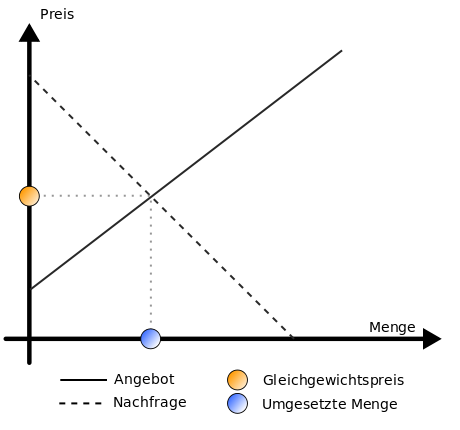
\includegraphics[width=0.28\textwidth]{pictures/lf01-pic/lf01-gleichgewichtspreis.png}
	\end{center}
	\caption{Entstehung des Gleichgewichtspreis}
\end{wrapfigure}
%%% Ende: Bild

Die Angebotslinie startet mit kleinem Angebot bei einem niedrigen Minimalpreis und wächst mit steigendem Preis. Die Nachfragelinie startet mit einer kleinen Nachfrage bei einem hohen Maximalpreis und nimmt mit fallendem Preis immer weiter an Menge zu. Wie an diesen zwei Linien zu erkennen ist, gibt es immer mehr Anbieter und Ware je höher der verlangte Preis ist. Umgekehrt gibt es immer mehr Abnehmer, die immer mehr kaufen, je niedriger der für die Ware verlangte Preis ist. Da die Preiswünsche von Anbietern und Abnehmern gegenläufig sind, stellt sich im Markt ein Gleichgewicht an der Schnittstelle von Angebot und Nachfrage ein, die den Gleichgewichtspreis und das Maximum des Umsatzes festlegt.

Marktsättigung führt dazu, dass kontinuierlich neue Produkte entwickelt werden müssen. Ein hilfreiches Instrument, um eine dauerhafte Marktsättigung zu umgehen, ist die geplante Obsoleszenz. Es werden absichtlich Bauteile verwendet, die nur eine begrenzte Lebenszeit haben; idealerweise beträgt die Lebenszeit eines solchen Bauteils nicht länger als die gesetzlich vorgeschriebene Garantiezeit. Dadurch wird eine konstante Nachfrage generiert.

%%% Ende: Einführung
%%%%%%%%%%%%%%%%%%%%%%%%%%%%%%%%%%%%%%%%%%%%%%%%%%%%%%%%%%%%%%%%%%%%%%%%%%%%%%%%

%%% Anfang: Werbung
\subsection{Werbung}

Was versteht das Recht unter sogenannten \ql Lockangeboten\qr? Welche Art von Werbung ist erlaubt und welche nicht? Diese und weitere Fragen werden in diesem Abschnitt beantwortet. 

Für beworbene Waren gilt eine Vorratsfrist von zwei Tagen. In Ausnahmen darf diese auch weniger getragen, beispielsweise wenn die Höhe der Nachfrage nicht absehbar war. Die Formulierung \ql Solange der Vorrat reicht\qr\ hebelt die Vorratsfrist aus, aber nur falls keine Vorerfahrung über die Höhe der Nachfrage bestand. Der Zweck von Lockangeboten besteht darin, Kunden in den Laden zu locken. Diese kommen bereits mit einer Kaufabsicht in den Laden. Wenn dann das beworbene Angebot nicht mehr erhältlich ist, greifen viele dieser Kunden zu einem ähnlichen aber teureren Produkt. Vergleichende Werbung ist nur in wenigen Fällen unproblematisch, sodass meistens darauf verzichtet wird. Unter {\bf Mondpreiswerbung} wird eine künstliche Erhöhung des Preises verstanden, um anschließend mit einer Reduzierung des Preises zu werden. Preise müssen normalerweise 6 Monate lang konstant bleiben. Außerdem fällt unzumutbare Belästigung in den Bereich des unlauteren Wettbewerbs.

Das Gesetz gegen unlauteren Wettbewerb (UWG) regelt, welche Formen der Werbung erlaubt sind und unter welchen Umständen sie als unlauter gelten. Im Einzelnen wurden die Paragraphen 3 bis 7 des UWG besprochen. Die Überschriften der Paragraphen lauten:

\begin{itemize}
	\item[§3] Verbot unlauterer geschäftlicher Handlungen
	\begin{itemize}
		\item Interessen von Mitbewerbern, Verbrauchern oder sonstigen Marktteilnehmern dürfen nicht spürbar beeinträchtigt werden.
		\item Geschäftliche Handlungen gegenüber Verbrauchern sind unzulässig, wenn sie nicht der für den Unternehmer geltenden fachlichen Sorgfalt entsprechen.
		\item Die Fähigkeit des Verbrauchers, sich auf Grund von Informationen zu entscheiden, darf nicht spürbar beeinträchtigt werden. Er darf nicht zu einer geschäftlichen Entscheidung veranlasst werden, die er sonst nicht getroffen hätte.
	\end{itemize}
	\item[§4] Beispiele unlauterer geschäftlicher Handlungen
	\begin{enumerate}
		\item Entscheidungsfreiheit der Marktteilnehmer durch Ausübung von Druck, in menschenverachtender Weise oder durch sonstigen unangemessenen unsachlichen Einfluss zu beeinträchtigen.
		\item Ausnutzen von geistigen oder körperlichen Gebrechen, des Alters, der geschäftlichen Unerfahrenheit, der Leichtgläubigkeit, der Angst oder der Zwangslage des Marktteilnehmers
		\item Verschleierung des Werbecharakters geschäftlicher Handlungen
		\item Bedingungen für die Inanspruchnahme von Verkaufsförderungsmaßnahmen wie Preisnachlässen, Zugaben oder Geschenken werden nicht klar und eindeutig angegeben
		\item Teilnahmebedingungen werden bei Preisausschreiben oder Gewinnspielen mit Werbecharakter nicht klar und eindeutig angegeben
		\item Teilnahme von Verbrauchern an einem Preisausschreiben oder einem Gewinnspiel ist an den Erwerb einer Ware oder die Inanspruchnahme einer Dienstleistung abhängig. \\
{\it Ausnahme:} Das Preisausschreiben oder Gewinnspiel ist naturgemäß mit der Ware oder Dienstleistung verbunden
		\item Die Kennzeichen, Waren, Dienstleistungen, Tätigkeiten oder persönlichen geschäftlichen Verhältnisse eines Mitbewerbers werden herabgesetzt oder verunglimpft			
		\item über die Waren, Dienstleistungen oder das Unternehmen eines Mitbewerbers oder über Unternehmer oder ein Mitglied der Unternehmensleitung Tatsachen behaupten oder verbreiten, die geeignet sind, den Betrieb des Unternehmens oder den Kredit des Unternehmers zu schädigen, sofern die Tatsachen nicht erweislich wahr sind.
	\end{enumerate}
	\item[§5] Irreführende geschäftliche Handlungen
	\begin{itemize}
		\item Eine geschäftliche Handlung ist Irreführend, wenn sie unwahre Angaben enthält oder sonstige zur Täuschung geeigneten Angaben über die wesentlichen Merkmale der Ware oder Dienstleistung oder den Anlass des Verkaufs enthält
		\item Verwechslungsgefahr mit einer anderen Ware oder Dienstleistung oder mit der Marke oder einem anderen Kennzeichen eines Mitbewerbers wird hervorgerufen
		\item Werbung mit einer Herabsetzung eines Preises, sofern der Preis nur eine unangemessen kurze Zeit gefordert worden ist ({\it Mondpreiswerbung})
	\end{itemize}
	\item[§5a] Irreführung durch Unterlassung
	\begin{itemize}
		\item Beeinflussung der Entscheidungsfähigkeit der Marktteilnehmer durch verschweigen wesentlicher Informationen
	\end{itemize}
	\item[§6] Vergleichende Werbung
	\begin{itemize}
		\item Vergleich bezieht sich nicht auf Waren oder Dienstleistungen für den gleichen Bedarf oder dieselbe Zweckbestimmung
		\item Nicht objektive auf wesentliche, relevante, nachprüfbare und typische Eigenschaften oder den Preis bezogen ist
		\item Verwechslung mit Mitbewerbern oder von diesen angebotenen Produkten
		\item Ruf des von einem Mitbewerber verwendeten Kennzeichen wird in unlauterer Weise ausgenutzt oder beeinträchtigt
		\item Ware oder Dienstleistung als Imitation oder Nachahmung einer unter einem geschützten Kennzeichen vertriebenen Ware oder Dienstleistung darstellen
	\end{itemize}
	\item[§7] Unzumutbare Belästigung
	\begin{itemize}
		\item Werbung, obwohl erkennbar ist, dass der angesprochene Marktteilnehmer diese Werbung nicht wünscht
		\item Werbung mit einem Telefonanruf gegenüber einem Verbraucher ohne dessen vorherige ausdrückliche Einwilligung
		\item Werbung unter Verwendung einer automatischen Anrufmaschine, eines Faxgeräts oder elektronischer Post, ohne vorherige ausdrückliche Einwilligung des Adressaten
		\item Verschleierung der Identität des Absenders
	\end{itemize}
\end{itemize}

%%% Ende: Werbung
%%%%%%%%%%%%%%%%%%%%%%%%%%%%%%%%%%%%%%%%%%%%%%%%%%%%%%%%%%%%%%%%%%%%%%%%%%%%%%%%

%%% Anfang: Bedürfnisse
\subsection{Bedürfnisse, Bedarf und Nachfrage}

\paragraph{Bedürfnisse}~\\
Unter einem Bedürfnis versteht man ein persönliches Mangelempfinden mit dem Bestreben, dieses zu beseitigen.

\begin{itemize}
\setlength\itemsep{0em}
	\item \textbf{Existenzbedürfnisse:} Lebensnotwendige Grundbedürfnisse des Menschen
	\item \textbf{Kulturbedürfnisse:} Teilnahme am gesellschaftlichen und kulturellen Leben. Sie sind nicht lebensnotwendig, erreichen jedoch in einer modernen Gesellschaft den Charakter von Muss-Bedürfnissen.
	\item \textbf{Luxusbedürfnisse:} Im Grunde überflüssige Dinge. Es werden Kann-Bedürfnisse mit Luxusgütern befriedigt. Mann muss sie nicht haben, jedoch ist es angenehm, wenn man sie sich leisten kann.
	\item \textbf{offene Bedürfnisse:}Bedürfnisse, die dem Menschen bewusst sind
	\item \textbf{Latente Bedürfnisse:}Unbewusste Bedürfnisse, die dem Menschen zunächst unbekannt sind und erst durch seine Umwelt geweckt werden
\end{itemize}
	
	
\paragraph{Bedarf}~\\
Der Bedarf ist die Summe der mit Kaufkraft ausgestatteten Bedürfnisse.

\begin{itemize}
\setlength\itemsep{0em}
	\item \textbf{Individualbedarf:} Bedarfsform, die für jede Einzelperson jeweils unterschiedliche Inhalte hat
	\item \textbf{Kollektivbedarf:} Bedarfsform, die für eine größere Anzahl von Personen in gleicher Weise besteht.
\end{itemize}
	
\paragraph{Nachfrage}~\\
Die Nachfrage ist der Teil des Bedarfs, der tatsächlich am Markt nachgefragt wird, also die Bedürfnisse, die mit Kaufkraft gedeckt sind und bei denen der Wille zur Befriedigung besteht.
	
%%% Ende: Bedürfnisse
%%%%%%%%%%%%%%%%%%%%%%%%%%%%%%%%%%%%%%%%%%%%%%%%%%%%%%%%%%%%%%%%%%%%%%%%%%%%%%%%

%%% Anfang: Betriebliche Kennzahlen
\subsection{Betriebliche Kennzahlen}

Als Kennziffern werden Indikatoren zur Bestimmung des wirtschaftlichen Erfolges bezeichnet, welche in Form von Zahlen ermittelt werden können. Dazu gehören offensichtliche Werte wie der Gewinn eines Unternehmens als auch die Produktivität. Betriebliche Kennzahlen können unter anderem in Relation zum Vorjahr, der Auslastung oder der Konkurrenz betrachtet werden.\\

Die {\bf Produktivität} ist eine Messgröße für die Ergiebigkeit der in der Produktion eingesetzten Produktionsfaktoren. {\bf Arbeitsproduktivität} misst analog zur Produktivität die Ergiebigkeit der eingesetzten Arbeitszeit. Bei der Berechnung der {\bf Wirtschaftlichkeit} handelt es sich um eine Erweiterung der Produktivität um den Faktor Geld. Zur Berechnung der Wirtschaftlichkeit werden die wertmäßigen Leistungen auf den Wert der eingesetzten Produktionsfaktoren bezogen. Die Erzielung von Gewinnen ist das Ziel privatwirtschaftlicher Unternehmen. Zur Beurteilung des Erfolges muss der Gewinn in Bezug zum eingesetzten Kapital gesetzt werden.\\

\begin{tabular}{lll}
Produktivität & $=$ & $\frac{mengenmässige\ Ausbringungsmenge}{mengenmässigen\ Einsatz\ der\ Produktionsfaktoren}$\\
& $=$ & $\frac{Output}{Input}$\\
Arbeitsproduktivität & $=$ & $ \frac{mengenmässige\ Ausbringungsmenge}{Arbeitsstunden}$\\
Wirtschaftlichkeit & $=$ & $\frac{Leistungen}{Kosten}$\\
\end{tabular}\\\\
 
Wie gut ein Unternehmen wirtschaftet, zeigt sich anhand seiner {\bf Rentabilität} (Eigen-/ Fremdkapitalrentabilität). Zur Erzielung von Gewinn aus dem eingesetzten Fremdkapital muss die Eigenkapitalrentabilität über dem Fremdkapitalzins liegen. Die {\bf Gesamtkapitalrentabilität} zeigt an, wie sich das gesamte in der Unternehmung eingesetzte Kapital verzinst.\\

\begin{tabular}{lll}
Eigenkapitalrentabilität & $=$ & $\frac{Gewinn\ \times\ 100}{Eigenkapital}$\\
Gesamtkapitalrentabilität & $=$ & $\frac{(Gewinn\ +\ Fremdkapital)\ \times\ 100}{Eigenkapitel\ +\ Fremdkapital}$	\\
\end{tabular}\\\\

Die {\bf Eigenkapitalquote} setzt das Eigenkapital in Bezug zum Gesamtkapital des Unternehmens. Die {\bf Fremdkapitalquote} setzt entsprechend das eingebrachte Fremdkapital in Bezug zum Gesamtkapital des Unternehmens. Ebenfalls von Bedeutung ist der {\bf Verschuldungsgrad}. Der Verschuldungsgrad. gibt den Anteil des Fremdkapitals am Eigenkapital an.\\

\begin{tabular}{lll}
Eigenkapitalquote & $=$ & $\frac{Eigenkapital\ \times\ 100}{Gesamtkapital}$\\
Fremdkapitalquote & $=$ & $\frac{Fremdkapital\ \times\ 100}{Gesantkapital}$\\
Verschuldungsgrad & $=$ & $\frac{Fremdkapital\ \times\ 100}{Eigenkapital}$\\
\end{tabular}\\\\

Die {\bf Anlageintensität} gibt den Anteil des Anlagevermögens (dem Unternehmen dauerhaft dienend) am Gesamtvermögen an. Die {\bf Arbeitsintensität} gibt den Anteil des Umlaufvermögens (dem Unternehmen kurzzeitig dienend, z.B. auf Lager liegende Waren) am Gesamtvermögen an.\\

\begin{tabular}{lll}
Anlageintensität & $=$ & $\frac{Anlagevermögen * 100}{Gesamtvermögen}$\\ 
Arbeitsintensität & $=$ & $\frac{Umlaufvermögen * 100}{Gesamtvermögen}$\\
\end{tabular}\\\\

Der {\bf Anlagendeckungsgrad I} gibt an, welcher Anteil des Anlagevermögens durch Eigenkapital gedeckt ist. Nach der {\it Goldenen Bilanzregel im engeren Sinne} sollte das Anlagevermögen durch Eigenkapital finanziert werden. Der {\bf Anlagendeckungsgrad II} gibt an, welcher Anteil des Anlagevermögens durch Eigenkapital und langfristiges Fremdkapital gedeckt ist. Nach der {\it Goldenen Bilanzregel im weiteren Sinne} soll die Finanzierung durch langfristig zur Verfügung stehendes erfolgen.\\

\begin{tabular}{lll}
Anlagedeckungsgrad I & $=$ & $\frac{Eigenkapital}{Anlagevermögen}$\\
Anlagedeckungsgrad II & $=$ & $\frac{Eigenkapital + langfristiges Fremdkapital}{Analgevermögen}$\\
\end{tabular}\\\\

Die {\bf Liquidität} ist eine Existenzbedingung des Unternehmens, die auch kurzfristig immer gesichert sein muss, um eine Zahlungsfähigkeit zu gewährleisten und eine eventuelle Gefahr für den Fortbestand durch Zahlungsunfähigkeit zu verhindern. Bei {\it flüssige Mittel} handelt es sich beispielsweise um Kassenbestände, Postgiroguthaben, Guthaben bei Kreditinstituten, Schecks, diskontfähige Wechsel und börsengängige Wertpapiere. 
Als {\it kurzfristige Forderungen} werden solche Forderungen mit einer Restlaufzeit von bis zu einem Jahr bezeichnet. {\it Kurzfristige Verbindlichkeiten} sind analog dazu Verbindlichkeiten mit einer Restlaufzeit von bis zu einem Jahr.\\

\begin{tabular}{lll}
Liquidität 1. Grades & $=$ & $\frac{Flüssige\ Mittel\ \times\ 100}{Kurzfristige\ Verbindlichkeiten}$\\
Liquidität 2. Grades & $=$ & $\frac{(Flüssige\ Mittel\ +\ kurzfr.\ Forderungen) \times\ 100}{Kurzfristige\ Verbindlichkeiten}$\\
Liquidität 3. Grades & $=$ & $\frac{Umlaufvermögen\ \times\ 100}{Kurzfristige\ Verbindlichkeiten}$
\end{tabular}

%%% Ende: Betriebliche Kennzahlen
%%%%%%%%%%%%%%%%%%%%%%%%%%%%%%%%%%%%%%%%%%%%%%%%%%%%%%%%%%%%%%%%%%%%%%%%%%%%%%%%

%%% Anfang: Preisfindung
\subsection{Preisfindung}

Manchmal werden Preise mit negativem Deckungsbeitrag -- das sind Preise, die unter den Produktionskosten liegen -- ausgeschrieben, um beispielsweise eine stärkere Marktdurchdringung oder eine Verdrängung von Konkurrenz zu erreichen. Ein negativer Deckungsbeitrag wird auch verwendet, um seine Lagerbestände zu leeren.

%%% Ende: Preisfindung
%%%%%%%%%%%%%%%%%%%%%%%%%%%%%%%%%%%%%%%%%%%%%%%%%%%%%%%%%%%%%%%%%%%%%%%%%%%%%%%%

%%% Anfang: Wirtschaftskreislauf
\subsection{Wirtschaftskreislauf}

Der Wirtschaftskreislauf beschreibt den Austausch von Gütern, Dienstleistungen und Geld. Dadurch werden die Zusammenhänge der einzelnen Akteure (Unternehmen, Haushalte, Banken, Staaten \dots) deutlich. 

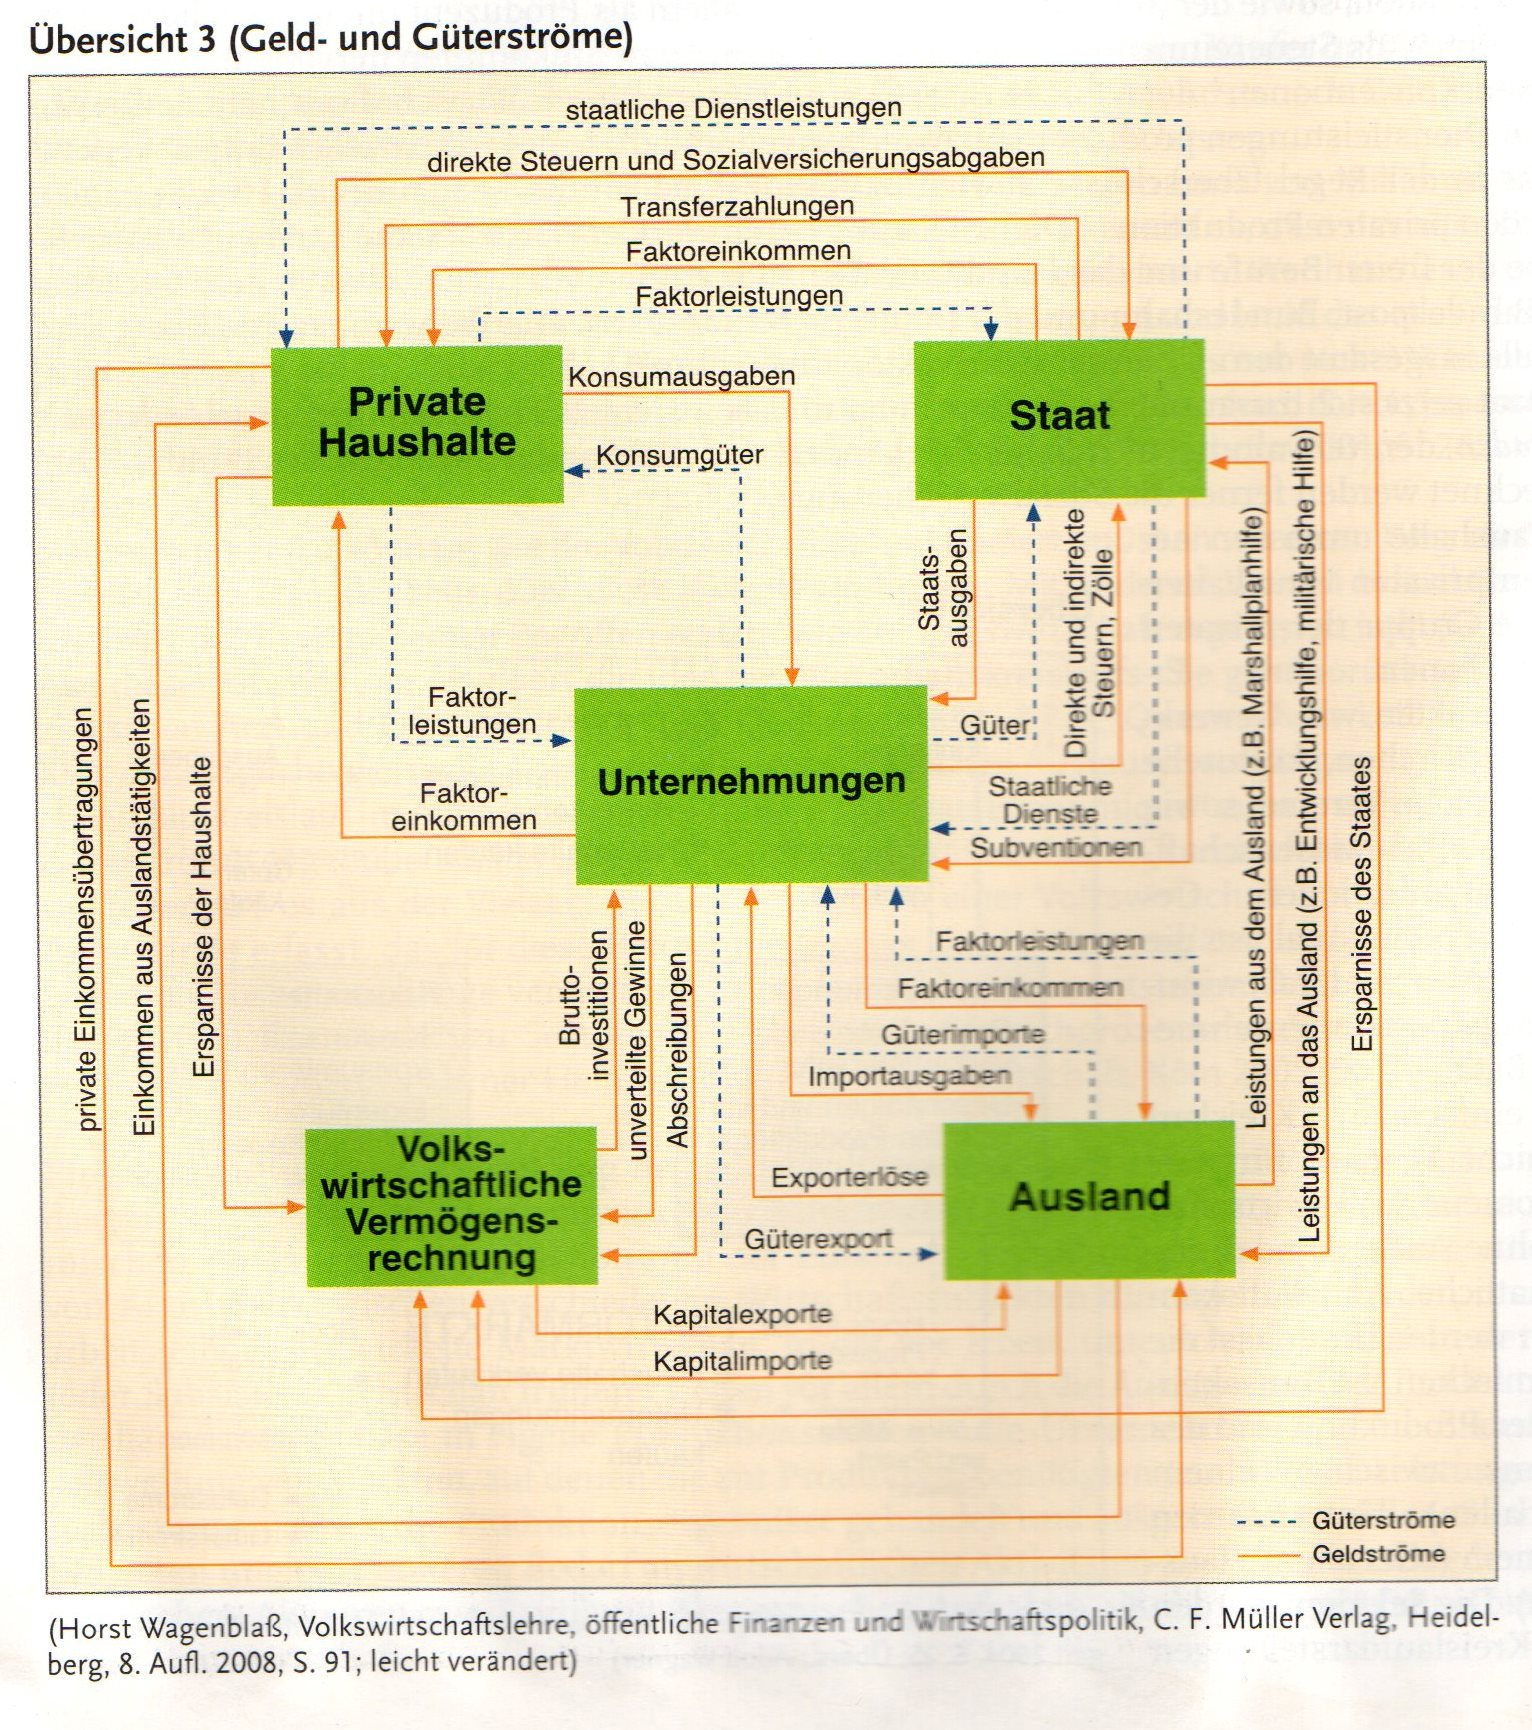
\includegraphics[scale=1.0]{pictures/lf01-pic/lf01-wirtschaftskreislauf.jpg}

%%% Ende: Wirtschaftskreislauf
%%%%%%%%%%%%%%%%%%%%%%%%%%%%%%%%%%%%%%%%%%%%%%%%%%%%%%%%%%%%%%%%%%%%%%%%%%%%%%%%

%%% Anfang: Staat
\subsection{Der Staat: soziale Marktwirtschaft:}

Der Staat soll die Freiheit aller Marktteilnehmer schützen und zugleich für soziale Gerechtigkeit sorgen. Möglichkeiten zum Eingriff in die Marktwirtschaft ergeben sich durch die Mittel der Fiskal-, Ordnungs-, Konjunktur- und Sozialpolitik. Bei Eingreifen in die Marktwirtschaft muss der Staat vier Ziele berücksichtigen. Diese Ziele werden auch als {\it magisches Viereck} bezeichnet, da sich niemals alle Ziele voll erreichen lassen.\\\\
\begin{tabular}{ll}
1. Stabilität des Preisniveaus & 2. hoher Beschäftigungsstand\\
3. außen-wirtschaftliches Gleichgewicht & 4. Wirtschaftswachstum\\
\end{tabular}

\begin{itemize}
\setlength\itemsep{0em}
	\item {\bf Fiskalpolitik:} Staat unterstützt viele Wirtschaftszweige (Subventionen); die Nachfrage wird durch erhöhen/senken der Steuern beeinflusst
	\item {\bf Ordnungspolitik:} Staat versucht die freie Marktwirtschaft zu schützen
	\item {\bf Konjunkturpolitik:} Stabilisierung der Wirtschaftsentwicklung
	\item {\bf Sozialpolitik:} sozialer Frieden soll gesichert werden; Unterstützung bestimmter Bevölkerungsgruppen (Sozialhilfe, Wohngeld)
\end{itemize}
	
%%% Ende: Staat
%%%%%%%%%%%%%%%%%%%%%%%%%%%%%%%%%%%%%%%%%%%%%%%%%%%%%%%%%%%%%%%%%%%%%%%%%%%%%%%%

%%% Anfang: Marktstrukturen und ihre Auswirkungen
\subsection{Marktstrukturen und ihre Auswirkungen}

Was ist ein Markt? Märkte sind Orte, an denen Angebot und Nachfrage aufeinandertreffen und durch den Ausgleich von Angebot und Nachfrage bildet sich ein Preis. Es gibt verschiedene Arten von Märkten, zum einen {\bf Faktormärkte} -- bspw. Arbeitsmarkt -- und zum anderen {\bf Gütermärkte}. Daneben gibt es noch verschieden Marktformen:

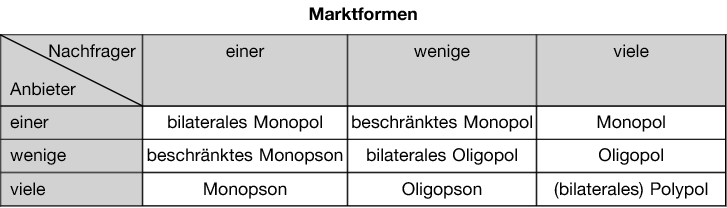
\includegraphics[scale=0.6]{pictures/lf01-pic/lf01-marktformen.png}

%%% Anfang: Markstrukturen > Prinzipien
\subsubsection{Ökonomische Prinzipien}

\begin{itemize}
\setlength\itemsep{0em}
	\item \textbf{Minimalprinzip:} Mit möglichst wenigen Mitteln ein gegebenes Ziel erreichen
	\item \textbf{Maximalprinzip:} Mit gegeben Mitteln den möglichst großen Nutzen erzielen
\end{itemize}

%%% Anfang: Marktstrukturen > Verhalten
\subsubsection{Anbieter- und Nachfragerverhalten}
Das Verhalten von Anbietern und Nachfragern stellen Einflussfaktoren auf den Märkten dar.

\begin{itemize}
	\setlength\itemsep{0em}
	\item {\bf Einflussfaktoren auf Seiten der Anbieter:}
	\begin{itemize}
	\setlength\itemsep{0em}
		\item Kosten der Produktionsfaktoren
		\item Gewinnerwartung
		\item Preis des Angebots
		\item Preis der Konkurrenz
		\item Stand der technischen Entwicklung
	\end{itemize}
	\item {\bf Einflussfaktoren auf Seiten der Nachfrager:}
	\begin{itemize}
	\setlength\itemsep{0em}
		\item Art und Dringlichkeit der Nachfrage
		\item Preis des nachfragten Gutes
		\item Preise der Konkurrenz
		\item Höhe der Kaufkraft
		\item Zukunftserwartungen der Konsumenten
	\end{itemize}
\end{itemize}

%%% Anfang: Marktstrukturen > Vollkommener Markt
\subsubsection{Vollkommener Markt}

Bei dem vollkommenen Markt handelt es sich um eine theoretische Vereinfachung der Realität. Der vollkommene Markt erfüllt folgende fünf Bedingungen:

\begin{enumerate}
\setlength\itemsep{0em}
	\item Rationales Verhalten aller Teilnehmer
	\item Homogenität aller Güter
	\item Keine Präferenzen der Teilnehmer
	\item Vollständige Markttransparenz
	\item Unendliche Reaktionsgeschwindigkeit der Teilnehmer
\end{enumerate}

Durch diese Optimalisierung der Realität gibt es nahezu nur unvollkommene Märkte. Dem vollkommenen Markt am nächsten kommt die Börse. Unter den Annahmen, dass vollständige Konkurrenz herrscht und dass Angebot und Nachfrage bloß vom Preis abhängen, gilt: (1) Wenn der Preis steigt, sinkt die Nachfrage \& (2) Wenn der Preis steigt, dann steigt das Angebot.

\subsubsection{Auswirkung der Veränderung von Angebot und Nachfrage}

Ein Marktgleichgewicht wird durch Veränderungen des Angebots oder der Nachfrage aufgehoben. Es entsteht ein neues Marktgleichgewicht mit einem neuen Gleichgewichtspreis und einer neuen Gleichgewichtsmenge. Unten sind die Auswirkungen der Veränderungen aufgelistet. [GRAFIKEN ERGÄNZEN]

\begin{itemize}
\setlength\itemsep{0em}
	\item Veränderung des Angebots
	\begin{itemize}
		\item {\bf Erhöhung des Angebots} bei gleichbleibender Nachfrage durch:
		\begin{itemize}
			\item Verringerung der Produktionkosten
			\item optimistische Zukunftserwartungen der Unternehmen
		\end{itemize}
		\item Wirkungen
		\begin{itemize}
			\item Verschiebung der Angebotskurve nach rechts
			\item Neues Marktgleichgewicht {\bf niedrigerem Gleichgewichtspreis} und {\bf höherer Gleichgewichtsmenge}
		\end{itemize}
		\item {\bf Verringerung des Angebots} bei gleichbleibender Nachfrage durch:
		\begin{itemize}
			\item Erhöhung der Produktionkosten
			\item pessimistische Zukunftserwartungen der Unternehmen
		\end{itemize}
		\item Wirkungen
		\begin{itemize}
			\item Verschiebung der Angebotskurve nach links
			\item Neues Marktgleichgewicht {\bf höherem Gleichgewichtspreis} und {\bf niedrigerer Gleichgewichtsmenge}
		\end{itemize}
	\end{itemize}
	\item Veränderung der Nachfrage
	\begin{itemize}
		\item {\bf Erhöhung des Nachfrage} bei gleichbleibendem Angebot durch:
		\begin{itemize}
			\item Einkommenserhöhung
			\item Steuersenkung
		\end{itemize}
		\item Wirkungen
		\begin{itemize}
			\item Verschiebung der Nachfragekurve nach rechts
			\item Neues Marktgleichgewicht {\bf höherem Gleichgewichtspreis} und {\bf höherer Gleichgewichtsmenge}
		\end{itemize}
		\item {\bf Verringerung des Nachfrage} bei gleichbleibendem Angebot durch:
		\begin{itemize}
			\item Einkommensrückgang
			\item Steuererhöhungen
		\end{itemize}
		\item Wirkungen
		\begin{itemize}
			\item Verschiebung der Nachfragekurve nach links
			\item Neues Marktgleichgewicht {\bf niedrigerem Gleichgewichtspreis} und {\bf niedrigerer Gleichgewichtsmenge}
		\end{itemize}
	\end{itemize}
\end{itemize}

%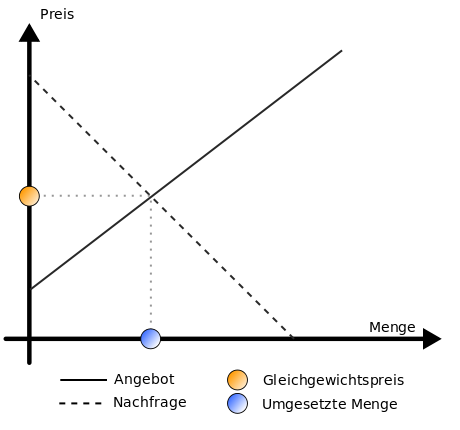
\includegraphics[scale=0.7]{pictures/lf01-pic/lf01-gleichgewichtspreis.png}\\
%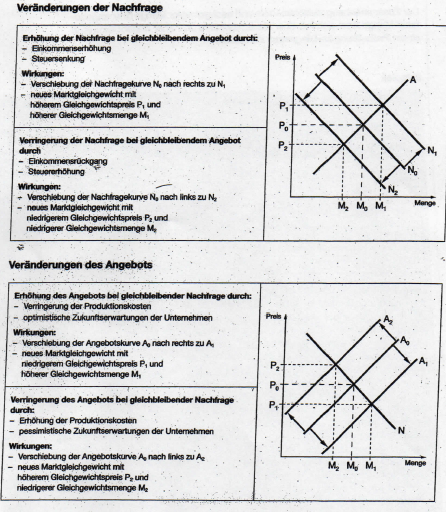
\includegraphics[scale=1.0]{pictures/lf01-pic/lf01-nachfrageverschiebung.png}

\noindent {\bf Preiselastizität} der Nachfrage gibt die Reaktionsempfindlichkeit der Nachfrage auf Preisveränderungen an.

%%% Ende: Marktsturkturen und ihre Auswirkungen
%%%%%%%%%%%%%%%%%%%%%%%%%%%%%%%%%%%%%%%%%%%%%%%%%%%%%%%%%%%%%%%%%%%%%%%%%%%%%%%%

%%% Anfang: Kooperation & Konzentration
\subsection{Kooperation \& Konzentration}

\begin{itemize}
\setlength\itemsep{0em}
	\item horizontale Kooperation
		\begin{itemize}
			\item Unternehmen gleicher Wirtschaftsstufe
			\item gleichartige Güter werden produziert
		\end{itemize}
	\item vertikale Kooperation
		\begin{itemize}
			\item Unternehmen unterschiedlicher Wirtschaftsstufen
		\end{itemize}
	\item anorganische Kooperation
		\begin{itemize}
			\item Unternehmen unterschiedlicher Wirtschaftsstufen und Branchen
		\end{itemize}
\end{itemize}

\begin{itemize}
\setlength\itemsep{0em}
	\item horizontale Konzentration
		\begin{itemize}
			\item Unternehmen gleicher Wirtschaftsstufe und Branche fusionieren zu einem Unternehmen
		\end{itemize}
	\item vertikale Konzentration
		\begin{itemize}
			\item Unternehmen unterschiedlicher Wirtschaftsstufen und gleicher Branche fusionieren zu einem Unternehmen
			\item Ein größerer Teil der Produktionskette kann von dem neuen Unternehemen verwirklicht werden
		\end{itemize}
	\item diagonale Konzentration
		\begin{itemize}
			\item Unternehmen unterschiedlicher Wirtschaftsstufen und Branchen fusionieren zu einem Unternehmen
			\item Ein Mischkonzern entsteht
			\item Es wird für Risikosträuung gesorgt
		\end{itemize}
\end{itemize}

%%% Ende: Kooperation & Konzentration
%%%%%%%%%%%%%%%%%%%%%%%%%%%%%%%%%%%%%%%%%%%%%%%%%%%%%%%%%%%%%%%%%%%%%%%%%%%%%%%%

%%% Anfang: Entgeltabrechnung
\subsection{Entgeltabrechnung}

%%% Anfang: Entgeltrechnung > Lohn
\subsubsection{Gehaltsbestandteile} 
Das Gehalt kann sich aus mehreren Faktoren zusammensetzen:
\begin{itemize}
\setlength\itemsep{0em}
	\item Grundlohn
	\item Naturallohn
		\begin{itemize}
			\item z.B. zusätzlich bei der Seeschiffahrt, im Nahrungsmittelbereich als \ql freie Kost und Logis\qr\
		\end{itemize}
	\item Zeitlohn
		\begin{itemize}
			\item Bezahlung auf Basis der geleisteten Arbeitszeit
		\end{itemize}
	\item Zuschlag
		\begin{itemize}
			\item Zuschläge für besondere Leistungen oder Belastungen des Arbeitsnehmers
			\item z.B. überstunden, Nachtarbeit, Spätschicht, Schmutzzuschlag, Hitzezuschlag, Kinderzuschlag, Ortszuschlag, Leistungszuschlag
		\end{itemize}
	\item Akkordlohn
		\begin{itemize}
			\item Bezahlung nach geleistetem Arbeitsergebnis unabhängig von der Arbeitszeit
		\end{itemize}
	\item Prämiensystem
		\begin{itemize}
			\item Zeitlohn und zusätzlich entsprechend der Leistung eine Prämie
		\end{itemize}
	\item Provision
		\begin{itemize}
			 \item Prozentuale Beteiligung am Wert der eigenen Geschäfte
		\end{itemize}
	\item Gratifikation
		\begin{itemize}
			\item Sonderzuwendung bei besonderen Anlässen
			\item z.B. Weihnachten, Jubiläum, Erreichung eines besonderen Ziels
		\end{itemize}
	\item Gewinnbeteiligung
		\begin{itemize}
			\item Beteiligung am Geschätsergebnis des Unternehmens
		\end{itemize}
	\item Vermögenswirksame Leistungen
		\begin{itemize}
			\item Ein Teil des Arbeitsverdienstes wird vermögenswirksam angelegt
			\item Arbeitgeber kann sich durch individuelle Vereinbarungen an den Beiträgen beteiligen
		\end{itemize}
	\item Aufwendungsersatz
		\begin{itemize}
			\item Aufwendungen des Arbeitnehmers müssen ersetzt werden
			\item z.B. Reisespesen oder Auslagen zur Beschaffung von Werkzeugen
		\end{itemize}
\end{itemize}

%%% Anfang: Entgeltrechnung > Abzüge
\subsubsection{Abzüge}
{\bf Faktoren}, die sich auf die Gehaltsabrechnung auswirken:
\begin{itemize}
\setlength\itemsep{0em}
	\item Einkommenshöhe: Die Lohnsteuer wird nur auf den Einkommensanteil oberhalb des Grundfreibetrages erhoben
	\item Familienstand: Aus dem Familienstand ergibt sich die Steuerklasse
	\item Kirchenmitgliedschaft
	\item Krankenkasse: Abhängig von der jeweiligen Krankenkasse werden Beiträge und variable Zusatzbeiträge fällig
	\item Wohnort: Vom Wohnort ist abhängig, ob ein Solidaritätszuschlag zu zahlen ist und wie hoch der Kirchensteuersatz liegt
\end{itemize}

\noindent Die Beiträge zur {\bf Sozialversicherung} werden zur Hälfte vom Arbeitgeber getragen (aktuelle Prozentwerte, 25.03.2015). Bei Azubis mit einem Gehalt unter 325\euro brutto übernimmt der Arbeitgeber die Versicherungsbeiträge vollständig.
\begin{itemize}
\setlength\itemsep{0em}
	\item Rentenversicherung (19,9\%)
	\item Pflegeversicherung (1,7\% + 0,25\% für Kinderlose ab 23 Jahren)
	\item Arbeitslosigkeit (4,2\%)
	\item Krankenkasse (variabel + 0,9\% Zusatzbeitrag für Arbeitnehmer)
\end{itemize}

\noindent {\bf Lohnsteuerklassen:}
\begin{itemize}
\setlength\itemsep{0em}
	\item[I]		ledig, geschieden, verwitwet
	\item[II]	Steuerklasse I mit min. einem Kind
	\item[III]	verheiratet, ein Verdiener
	\item[IV]	verheiratet, zwei Verdiener in IV, beide Verdienen etwa gleich viel
	\item[V]		verheiratet, zwei Verdiener, Partner in III, Verdienst ist unterschiedlich
	\item[VI]	mehrere Lohnsteuerkarten
\end{itemize}

%%% Anfang: Entgeltrechnung > Beispielrechnung
\subsubsection{Beispielabrechnung}

Voraussetzungen: Angestellte, ledig, 24 Jahre, 2.100\euro\ brutto.\\
\begin{tabular}{ll}
Lohnsteuer (Kl. I)			& $287,33$\euro\\
Kirchensteuersatz 			& $9\%$\\
Solidaritätszuschlag			& $5,5\%$\\
Krankenkasse					& allg. Beitragssatz: $13,8\%$\\
zusätzlicher Beitragssatz	& $0,9\%$\\
Rentenversicherung			& $19,5\%$\\
Arbeitslosenversicherung		& $4,5\%$\\
Pflegeversicherung			& $1,7\%$\\
\end{tabular}\newline

\noindent {\bf Rechnung:}\\
\begin{table}[!h]
\small
\begin{tabular}{lll}
Kirchensteuer				& $=$ & $Lohnsteuer\ \times\ Kirchensteuersatz$\\
							& $=$ & $287,33\textit{\euro}\ \times\ 9\% $\\
							& $=$ & $25,85\textit{\euro}$\\
Solidaritätszuschlag	 		& $=$ & $Lohnsteuer\ \times\ 5,5\%$\\
							& $=$ & $287,33\textit{\euro}\ \times\ 5,5\%$\\
							& $=$ & $15,80\textit{\euro}$\\
Krankenversicherung			& $=$ & $\frac{Bruttolohn\ \times\ Krankenversicherungssatz}{2}\ +\ Bruttolohn\ \times\ Zusatzbeitrag$\\
							& $=$ & $\frac{2100\textit{\euro}\ \times\ 13,8\%}{2}\ +\ 2100\textit{\euro}\ \times\ 9\%$\\
							& $=$ & $163,80\textit{\euro}$\\
Rentenversicherung			& $=$ & $\frac{Bruttolohn\ \times\ Rentenversicherungssatz}{2}$\\
							& $=$ & $\frac{2100\textit{\euro}\ \times\ 19,5\%}{2}$\\
							& $=$ & $204,75\textit{\euro}$\\
Arbeitslosenversicherung		& $=$ & $\frac{Bruttolohn\ \times\ Arbeitslosenversicherungssatz}{2}$\\
							& $=$ & $\frac{2100\textit{\euro}\ \times\ 4,5\%}{2}$\\
							& $=$ & $47,25\textit{\euro}$\\
Pflegeversicherung			& $=$ & $\frac{Bruttolohn\ \times\ Pflegeversicherungssatz}{2}\ +\ Bruttolohn\ \times\ Zusatzbeitrag$\\
							& $=$ & $\frac{2100\textit{\euro}\ \times\ 1,7\%}{2}\ +\ 2100\textit{\euro}\ \times\ 0,25\%$\\
							& $=$ & $23,10\textit{\euro}$\\
\end{tabular}
\end{table}

\begin{tabular}{lrl}
& $2.100,00\textit{\euro}$ & Brutto\\
$-$ & $287,33\textit{\euro}$ & Lohnsteuer\\
$-$ & $25,85\textit{\euro}$ & Kirchensteuer\\ 
$-$ & $15,80\textit{\euro}$ & Solidaritätszuschlag\\
$-$ & $163,80\textit{\euro}$ & Krankenversicherung\\
$-$ & $204,75\textit{\euro}$ & Rentenversicherung\\
$-$ & $47,25\textit{\euro}$ & Arbeitslosenversicherung\\
$-$ & $23,10\textit{\euro}$ & Pflegeversicherung\\
\hline
& $1.332,12\textit{\euro}$ & Netto\\
\end{tabular}


%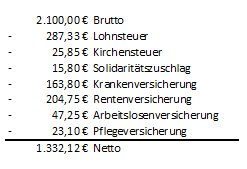
\includegraphics[scale=1.0]{pictures/lf01-pic/lf01-beispielentgeldabrechung.png}

%%% Ende: Entgeltabrechnung
%%%%%%%%%%%%%%%%%%%%%%%%%%%%%%%%%%%%%%%%%%%%%%%%%%%%%%%%%%%%%%%%%%%%%%%%%%%%%%%%

%%% Anfang: Rechts- und Geschäftsfähigkeit
\subsection{Rechts- und Geschäftsfähigkeit}

Wichtige Punkte, die in einem Kaufvertrag notiert werden sollten:

\begin{itemize}
\setlength\itemsep{0em}
	\item Art und Güte der Leistung
	\item Lieferzeit
	\item Verpackungs- und Versandkosten
	\item Zahlungsart
	\item Preis
	\item Erfüllungsort
\end{itemize}

%%% Anfang: > Rechtsordnung
\subsubsection{Rechtsordnung}
Die Rechtsordnung unterscheidet zwischen dem {\bf öffentlichen} und dem {\bf privaten Recht}. Das öffentliche Recht beschreibt die Rechtsbeziehungen zwischen den Einzelpersonen und dem Staat. Dies ist z. B. im Steuerrecht und im Strafrecht der Fall. Das private Recht beschreibt die Rechtsbeziehungen zwischen den Einzelpersonen, wie es z. B. im BGB und im Handelsgesetzbuch (HGB) der Fall ist.\newline

\noindent {\bf Rechtsfähigkeit} ist die Fähigkeit, Träger von Rechten und Pflichten zu sein. {\bf Natürliche Personen} sind von Geburt bis zu ihrem Tod rechtsfähig. {\bf Juristische Personen} (bspw. Vereine, Stiftungen, Handelsgesellschaften\dots ) sind dies erst mit Eintragung in das jeweilige Register (z.B. GmbH, AG).\newline

\noindent {\bf Geschäftsfähigkeit} ist die Fähigkeit, selbstständig und wirksam Rechtsgeschäfte abschließen zu können.

\begin{itemize}
\setlength\itemsep{0em}
	\item {\bf geschäftsunfähig} (Willenserklärungen sind nichtig)
	\begin{itemize}
		\item Kinder bis zum vollendeten 7. Lebensjahr
		\item geschäftsunfähige Personen (§ 104 BGB)
		\item {\it Ausnahmen:} volljährige Geschäftsunfähige, die Geschäfte des täglichen Lebens mit geringen Mitteln bewirken (§ 105 BGB)
	\end{itemize}
	\item {\bf beschränkt geschäftsfähig} (Willenserklärungen sind schwebend unwirksam)
	\begin{itemize}
		\item Kinder zwischen dem vollendeten 7. und vollendetem 18. Lebensjahr (§§ 106 bis 113 BGB)
		\item betreute Volljährige mit gerichtlichem Einwilligungsvorbehalt für bestimmte Handlungsbereiche. {\it Hinweis:} Der gesetzliche Vertreter kann auch nachträglich genehmeigen.
		\item Taschengeldgeschäfte nach § 110 BGB
		\item vorteilhafte Rechtsgeschäfte nach § 107 BGB
		\item selbstständiger Betrieb eines Erwerbsgeschäftes nach § 112 BGB
		\item genehmigte Arbeitsverhältnisse nach § 113 BGB
	\end{itemize}
	\item {\bf voll geschäftsfähig}: alle sonstigen volljährigen Personen
\end{itemize}

\noindent {\bf Deliktfähigkeit} (vgl. § 828 BGB) / {\bf Schuldfähigkeit} (vgl. § 19 StGB) bedeutet Verantwortung für unerlaubte Handlungen übernehmen zu müssen. Für deliktunfähige Personen gilt, dass die jeweilige Aufsichtsperson ihre Aufsichtspflicht zu beachten hat.

\begin{itemize}
\setlength\itemsep{0em}
	\item {\bf deliktunfähig}: Kinder bis zur Vollendung des 7. Lebensjahres
	\item {\bf beschränkt deliktfähig}: Minderjährige zwischen 7 und 18 Jahren und Taubstumme (Schuldfähigkeit ab 14 Jahren)
	\item {\bf voll deliktfähig}: Personen ab Vollendung des 18. Lebensjahres, sofern geschäftsfähig
\end{itemize}

%%% Anfang: > Rechtsgeschäfte
\subsubsection{Rechtsgeschäfte}

\paragraph{Rechtsgeschäfte durch Willenserklärung}~\\

\begin{itemize}
\setlength\itemsep{0em}
	\item Einseitige Rechtsgeschäfte: Eine Willenserklärung reicht zur Wirksamkeit; {\bf empfangsbedürftig}: z.B. Kündigung; {\bf nicht empfangsbedürftig}: z.B. Testament
	\item Mehrseitige Rechtsgeschäfte: Zwei oder meher übereinstimmende Willenserklärungen sind zur Wirksamkeit notwendig, z.B. Kauf-, Miet-, Arbeitsvertrag
	\item Vertretung und Vollmacht: Ein Vertreter kann im Rahmen der Vollmacht Rechtsgeschäfte für andere eingehen
	\item Grundsatz: Vertragsfreiheit; Vertragsschließende Parteien sind in den Vereinbarungen frei, wenn diese nicht gegen das Gesetz und Rechtsprechung verstoßen
\end{itemize}

\paragraph{Nichtige Verträge}~\\

\begin{itemize}
\setlength\itemsep{0em}
	\item Verträge mit Geschäftsunfähigen (§105 BGB)
	\item Vertreter verweigert Zustimmung mit beschränkt Geschäftsfähigen (§108 BGB)
	\item Verträge, die nur zum Schein abgeschlossen wurden ({\bf Scheingeschäftge}, §117 BGB)
	\item nicht ernst gemeinte Verträge ({\bf Scherzgeschäfte}, §118 BGB)
	\item Vertragserfüllung verstößt gegen geltendes Recht und Gesetz (§134 BGB)
	\item Verträge verstoßen gegen gute Sitten, z.B. Wucher (§138 BGB)
	\item Verstoß gegen Formvorschriften: Schriftform, notarielle Beurkundung, öffentliche Beglaubigunng (§125 BGB)
\end{itemize}

\paragraph{Anfechtbare Verträge}~\\

\begin{itemize}
\setlength\itemsep{0em}
	\item Erklärungsirrtum (§119 Abs 1 BGB): Vertragsbestandteil wird unwissentlich falsch erklärt oder falsch geäußert (Verschrieben, Versprechen)
	\item Übermittlungsirrtum (§120): unbewusste Falschübermittlung durch einen Dritten
	\item Eigenschaftsirrtum (§119 BGB Abs. 2 BGB): Irrtum über eine wesentliche Eigenschaft in der Sache oder in der Person
	\item Arglistige Täuschung (§123 Abs. 1 BGB): Es kann durch Tatsachen nachgewiesen werden, dass ein Vertragspartner arglistig (mit Vorsatz) getäuscht hat
	\item Widerrechtliche Drohung (§123 Abs. 2 BGB): Die Willenserklärung wurde durch Androhung eines Übels erzwungen
\end{itemize}

%%% Ende: Entgeltabrechnung
%%%%%%%%%%%%%%%%%%%%%%%%%%%%%%%%%%%%%%%%%%%%%%%%%%%%%%%%%%%%%%%%%%%%%%%%%%%%%%%%

%%% Anfang: Existenzgründung
\subsection{Existenzgründung}

%%%Anfang: Existenzgründung > Unternehmen, Firma und Betrieb
\subsubsection{Unternehmen, Firma und Betrieb}

{\bf Unternehmen} ist die rechtliche Bezeichnung für eine Unternehmung. Eine 	Unternehmung ist ein wirtschaftlich-rechtlich organisiertes Gebilde, welches es ein Ziel hat. Dieses ist meist die nachhaltige Leistungserzielung mit dem Effekt der Gewinnmaximierung.\\

\noindent {\bf Firma} ist rechtliche Begriff für den Namen, unter dem ein Kaufmann im Handel seine Geschäfte betreibt. Die Firma ist also der Name eines kaufmännischen Unternehmens. Zusatz neben der Firma ist die Rechtsform.\\

\noindent {\bf Betrieb} ist die rechtliche Bezeichnung für den tatsächlichen Ort, an dem Güter oder Dienstleistungen erstellt werden. Ein Betrieb ist somit die Produktionsstätte.

%%%Anfang: Existenzgründung > Gründen einer Unternehmung
\subsubsection{Gründen einer Unternehmung}
Durch die Gewerbefreiheit kann in Deutschland grundsätzlich jeder ein Unternehmen gründen. Ein Unternehmer muss jedoch die gesetzlichen Rahmenbedingungen beachten.

\paragraph{Voraussetzungen für die Gründung eines Unternehmens} ~\\

\begin{table}[!h]
\small
\begin{tabular}{lll}
	\parbox[t]{4.5cm}{
	{\bf Persönliche\\Voraussetzungen}
	\begin{itemize}
		\item Geschäftsfähigkeit
		\item Risikobereitschaft
		\item Aufgeschlossenheit gegenüber neuen Ideen
		\item Entscheidungsfähigkeit
		\item Kontaktfähigkeit
		\item Motivationsfähigkeit
		\item Kritikfähigkeit
		\item Durchhaltevermögen
	\end{itemize}
	} &
	\parbox[t]{4.5cm}{
	{\bf Sachliche und wirtschaftliche Voraussetzungen}
	\begin{itemize}
		\item Branchenkenntnisse
		\item Standortwahl
		\item Kapital
		\item Personal
		\item Ware
		\item Geschäftsverbindungen
	\end{itemize}
	} &
	\parbox[t]{4.5cm}{
	{\bf Rechtliche Voraussetzungen}
	\begin{itemize}
		\item Gewerbeanmeldung
		\item Anmeldung zur Eintragung ins Handelsregister
		\item Anmeldung beim Finanzamt
		\item Anmeldung bei der Berufsgenossenschaft
		\item Anmeldung bei der IHK
	\end{itemize}
	}
\end{tabular}
\end{table}

%%%Anfang: Existenzgründung > Kaufmannseigenschaft
\subsubsection{Kaufmannseigenschaft}
Im Sinne des Handelsgesetzbuches (HGB) ist Kaufmann, wer ein Handelsgewerbe betreibt. Ein Handelsgewerbe ist laut HGB jeder Gewerbebetrieb, der nach Art und Umfang einen in kaufmännischer Weise eingerichteten Geschäftsbetrieb erfordert. Personen, die ein Handelsgewerbe betreiben, sind Kaufleute kraft Gewerbebetrieb ({\bf Istkaufmann}). Personen, die einen Gewerbebetrieb betreiben, der keine kaufmännische Organisation erfordert, sowie Inhaber von land- und forstwirtschaftlichen Betrieben sind keine Kaufleute kraft Gewerbebetrieb. Sie können sich aber trotzdem in das Handelsregister eintragen lassen. Damit werden sie zu Kaufleuten ({\bf Kannkaufmann}). Ohne Rücksicht auf die Art des Gewerbes sind alle Kapitalgesellschaften und eingetragenen Genossenschaften zur Eintragung in das Handelsregister verpflichtet. Damit sind sie Kaufleute kraft Rechtsform ({\bf Formkaufmann}).

%%%Anfang: Existenzgründung > Handelsregister
\subsubsection{Handelsregister}
Das Handelsregister ist ein beim Amtsgericht geführtes amtliches Verzeichnis der Kaufleute eines Amtsgerichtsbezirks. Die Öffentlichkeit soll durch das Handelsregister über die grundlegenden Rechtsverhältnisse der Unternehmungen unterrichtet werden. Zudem wird dadurch die Firma des Kaufmanns geschützt. Das Handelsregister ist in zwei Abteilungen unterteilt:
\begin{itemize}
\setlength\itemsep{0em}
	\item {\bf Abteilung A} enthält die Einzelunternehmungen sowie die Personengesellschaften und
	\item {\bf Abteilung B} enthält die Kapitalgesellschaften.
\end{itemize}

\paragraph{Wirkung der Eintragungen}
\begin{itemize}
\setlength\itemsep{0em}
	\item Deklaratorische (rechtsbezeugende) Wirkung
	\begin{itemize}
		\item Rechtswirkung kann bereits vor der Eintragung eingetreten sein
		\item {\it Beispiel:} Eintragung der Prokura (schon vor der Eintragung wirksam)
	\end{itemize}
	\item Konstitutive (rechtserzeugende) Wirkung
	\begin{itemize}
		\item Rechtswirkung tritt erst durch die Eintragung ein
		\item {\it Beispiel:} Eintragung einer Aktiengesellschaft (AG ist vor der Eintragung eine GbR)
	\end{itemize}
\end{itemize}

\paragraph{Öffentlichkeit des Handelsregisters}~\\
Das Handelsregister ist öffentlich. Jeder hat das Recht, Einsicht in das Handelsregister zu nehmen.\footnote{Die IHK verlangt die Antwort: \ql Jeder, der ein begründetes Interesse hat, kann Einsicht nehmen.\qr} Die Eintragungen in das Handelsregister werden durch Veröffentlichung im Bundesanzeiger und in einer örtlichen Tageszeitung bekannt gemacht.

%%%Anfang: Existenzgründung > Firma
\subsubsection{Firma}

\paragraph{Firmenarten}
\begin{itemize}
\setlength\itemsep{0em}
	\item {\bf Personenfirma}: Die Firma besteht aus einem oder mehreren bürgerlichen Namen und der Rechtsformbezeichnung; {\it Beispiele:} Marc Mönning e.Kfm., Meurer und Lemloh KG
	\item {\bf Sachfirma}: Die Firma besteht aus dem Firmennamen, der aus dem Gegenstand des Unternehmens abgeleitet ist, und der Rechtsformbezeichnung; {\it Beispiele:} IT-Systemhaus Bonn GmbH, Kölner Umzugsservice KG
	\item {\bf Gemischte Firma}: Die Firma besteht aus den Personennamen und dem Gegenstand des Unternehmens und der Rechtsformbezeichnung; {\it Beispiele:} Schmitz Eiscreme GmbH, Reisebüro Nicole Schöneberger e.Kfr.
	\item {\bf Fantasiefirma}: Die Firma besteht aus einem frei erfundenen Firmennamen und der Rechtsformbezeichnung; {\it Beispiele:} Ruckzuck KG, Living with a box GmbH
\end{itemize}

\paragraph{Firmengrundsätze}~\\
Bei der Wahl der Firma müssen neben den gesetzlichen Vorschriften auch die folgenden Firmengrundsätze beachtet werden.

\begin{itemize}
\setlength\itemsep{0em}
	\item {\bf Firmenwahrheit:} Die Firma muss bei der Unternehmensgründung der Wahrheit entsprechen, bei einer Personenfirma müssen also bürgerlicher Name und Firma übereinstimmen
	\item {\bf Firmenklarheit:} Die Firma muss den Tatsachen entsprechen und darf nicht über Art und Umfang des Geschäfts täuschen
	\item {\bf Firmenöffentlichkeit:} Jeder Kaufmann ist verpflichtet, seine Firma im Handelsregister eintragen zu lassen
	\item {\bf Firmenausschließlichkeit:} Jede Firma muss sich von einer anderen Firma am selben Ort unterscheiden. Bei einer Personenfirma mit gleichem Familiennamen muss die Firma eine eindeutige Unterscheidung ermöglichen
	\item {\bf Firmenbeständigkeit:} Die Firma darf bei einem Inhaberwechsel beibehalten werden. Ein Zusatz in der Firma muss auf das Nachfolgeverhältnis hinweisen ({\it Beispiel:} IT-Service Steinkamp, Inhaber Rolf Schmitz)
\end{itemize}

%%% Anfang: Existenzgründung > Vollmachten
\subsubsection{Vollmachten}
Unter Vollmacht versteht man das Recht eines Mitarbeiters, im Namen und auf Rechnung des Unternehmens Rechtsgeschäfte abschließen zu können. Es wird zwischen Handlungsvollmacht und Prokura unterschieden.
	
%%% Anfang Existenzgründung > Vollmachten > Prokura
\paragraph{Prokura}~\\
Die Prokura ist die weitreichendste Vollmacht. Der Prokurist wird zu allen Rechtsgeschäften ermächtigt, die der Betrieb irgendeines Handelsgewerbes mit sich bringt. Sie ist im Außenverhältnis nicht beschränkbar.
	
\subparagraph{Umfang der Prokura} Ein Prokurist darf grundsätzlich alle {\bf gewöhnlichen} und {\bf außergewöhnlichen} Rechtsgeschäfte vornehmen. Er benötigt jedoch eine besondere Vollmacht zum Verkauf und zur Belastung von Grundstücken. Ein Prokurist darf nicht:
\begin{itemize}
\setlength\itemsep{0em}
	\item Prokura erteilen oder entziehen
	\item Bilanzen und Steuererklärungen unterzeichnen
	\item neue Gesellschafter aufnehmen
	\item Eröffnung eines Insolvenzverfahrens
	\item das Unternehmen auflösen oder veräußern
\end{itemize}
	
\subparagraph{Arten der Prokura}
\begin{itemize}
\setlength\itemsep{0em}
	\item {\bf Einzelprokura:} Der Prokurist darf die Prokura allein ausüben.
	\item {\bf Filialprokura:} Die Prokura wird auf die Geschäfte einer Unternehmensfiliale beschränkt.
	\item {\bf Gesamtprokura:} Die Vertretungsmacht darf nur von mehreren Prokuristen gemeinschaftlich ausgeübt werden
\end{itemize}
	
\subparagraph{Erteilung der Prokura} Die Prokura kann nur von einem Kaufmann erteilt werden.
	
\subparagraph{Unterschrift} Der Prokurist unterschreibt, indem der Firmenbezeichnung sein Name mit dem Zusatz    {\bf ppa.} (per procura) hinzugefügt wird.
	
\subparagraph{Beginn der Prokura} Im Innenverhältnis beginnt die Prokura mit ihrer Erteilung, im Außenverhältnis jedoch erst mit der Eintragung und Veröffentlichung im Handelsregister. Die Eintragung hat hier also deklaratorische Wirkung.
	
\subparagraph{Erlöschen der Prokura} Die Prokura erlischt mit der Beendigung des Rechtsverhältnisses, an das sie gebunden ist (z.B. Beschäftigungsverhältnis), durch Widerruf, durch die Auflösung des Geschäfts oder durch den Tod des Prokuristen.
	
%%% Anfang Existenzgründung > Vollmachten > Handlungsvollmacht
\paragraph{Handlungsvollmacht}~\\
Die Handlungsvollmacht erstreckt sich nur auf Rechtsgeschäfte, die in dem jeweiligen Handelsgewerbe {\bf gewöhnlich} vorkommen. Sie ist im Gegensatz zur Prokura beliebig einschränkbar. Ein Handlungsbevollmächtigter darf nicht:

\begin{itemize}
\setlength\itemsep{0em}
	\item Grundstücke veräußern oder belasten
	\item Darlehen aufnehmen
	\item Prozesse im Namen des Unternehmens führen
\end{itemize}
	
\subparagraph{Arten der Handlungsvollmacht}
\begin{itemize}
\setlength\itemsep{0em}
	\item {\bf Einzelvollmacht:} Bevollmächtigung zur Vornahme eines einzelnen Rechtsgeschäfts
	\item {\bf Artvollmacht:} Bevollmächtigung zur Vornahme einer bestimmten Art von Rechtsgeschäften
	\item {\bf allgemeine Handlungsvollmacht:} Bevollmächtigung zur Vornahme aller gewöhnlichen Rechtsgeschäfte, die in dem Handelsgewerbe des jeweiligen Geschäftszweigs vorkommen
\end{itemize}
	
\subparagraph{Unterschrift} Der Handlungsbevollmächtigte unterschreibt, indem er der Firmenbezeichnung seinen Namen mit dem Zusatz {\bf i.A.} (im Auftrag) oder {\bf i.V.} (in Vertretung) hinzufügt.
	
\subparagraph{Erteilung der Handlungsvollmacht} Die Handlungsvollmacht kann formlos von Kaufleuten und Prokuristen erteilt werden. Jeder Bevollmächtigte kann innerhalb seiner Vollmacht Untervollmachten erteilen. Handlungsvollmachten werden nicht in das Handelsregister eingetragen.
	
\subparagraph{Erlöschen der Handlungsvollmacht} Die Handlungsvollmacht erlischt mit der Beendigung des Rechtsverhältnisses, an das sie gebunden ist (z.B. Beschäftigungsverhältnis), durch Widerruf, mit Erledigung des Auftrags bei einer Einzelvollmacht, durch Auflösung des Geschäfts oder durch den Tod des Handlungsbevollmächtigten.
	
%%% Anfang Existenzgründung > Unternehmensformen
\subsubsection{Unternehmensformen}

Die Rechtsordnung stellt den Unternehmen verschiedene Unternehmensformen (Rechtsformen) zur Verfügung und überlässt es den Gründern oder Eigentümern, sich für eine bestimmte Rechtsform zu entscheiden.
	
%%% Anfang Existenzgründung > Unternehmensformen > Überblick
\paragraph{Überblick}~\\
Ein Unternehmen kann als Einzel- oder Gesellschaftsunternehmung betrieben werden. Die Gesellschaftsunternehmen lassen sich weiter unterteilen in Personen- und Kapitalgesellschaften. Die verschiedenen Unternehmensformen lassen sich auf Grund der Merkmale Gründung, Haftung, Mindestkapital, Firma und Gewinn- und Verlustteilung unterscheiden.\\
	
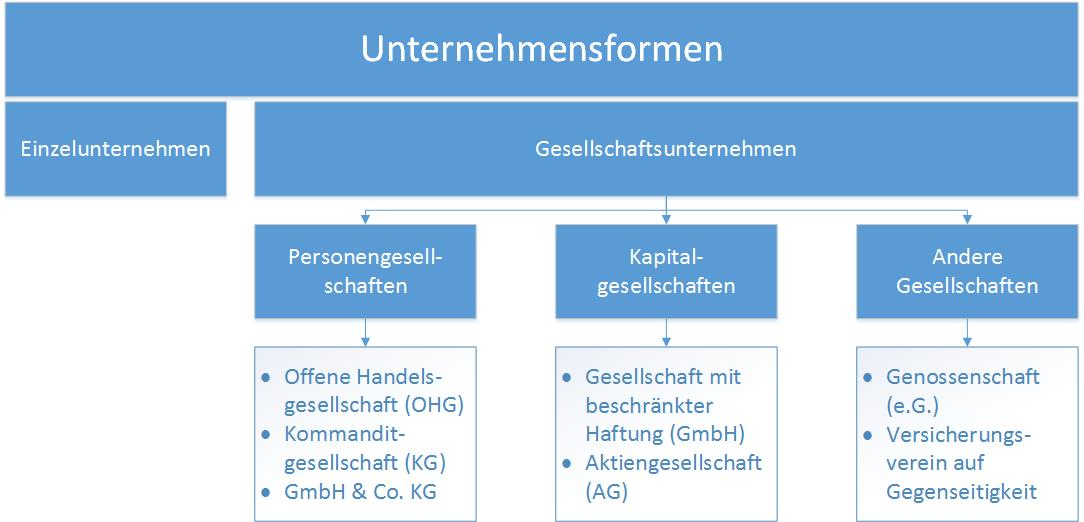
\includegraphics[scale=0.5]{pictures/lf01-pic/lf01-unternehmensueberblick.jpg}\newpage
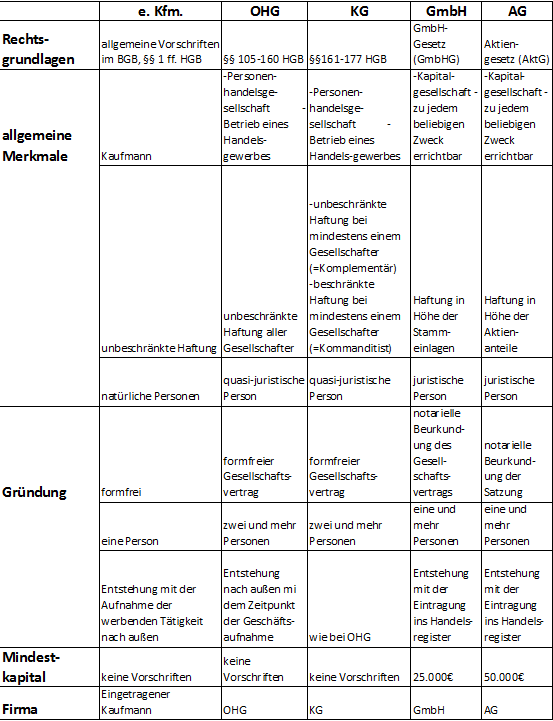
\includegraphics[scale=1.0]{pictures/lf01-pic/lf01-uebersicht_unternehmen_01.png}\newpage
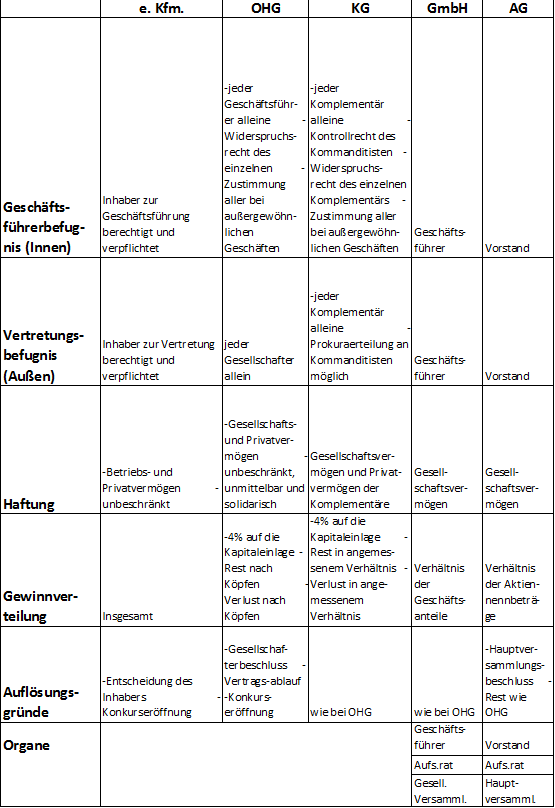
\includegraphics[scale=1.0]{pictures/lf01-pic/lf01-uebersicht_unternehmen_02.png}\newpage

%%% Ende: Existenzgründung
%%%%%%%%%%%%%%%%%%%%%%%%%%%%%%%%%%%%%%%%%%%%%%%%%%%%%%%%%%%%%%%%%%%%%%%%%%%%%%%%

%%% Anfang: Beschaffungsprozess
\subsection{Störungen im Beschaffungs- und Lieferungsprozess}
Mit dem Abschluss des Kaufvertrags haben Verkäufer und Käufer Pflichten übernommen. Der Verkäufer hat die Pflicht, zu liefern und der Käufer hat die Pflicht, das Gekaufte anzunehmen und zu bezahlen. In den folgenden Abschnitten wird geklärt, was passiert, wenn es beide diesen drei Pflichten zu Verzögerungen kommt und welche Möglichkeiten dem Verkäufer respektive Käufer offenstehen.\\

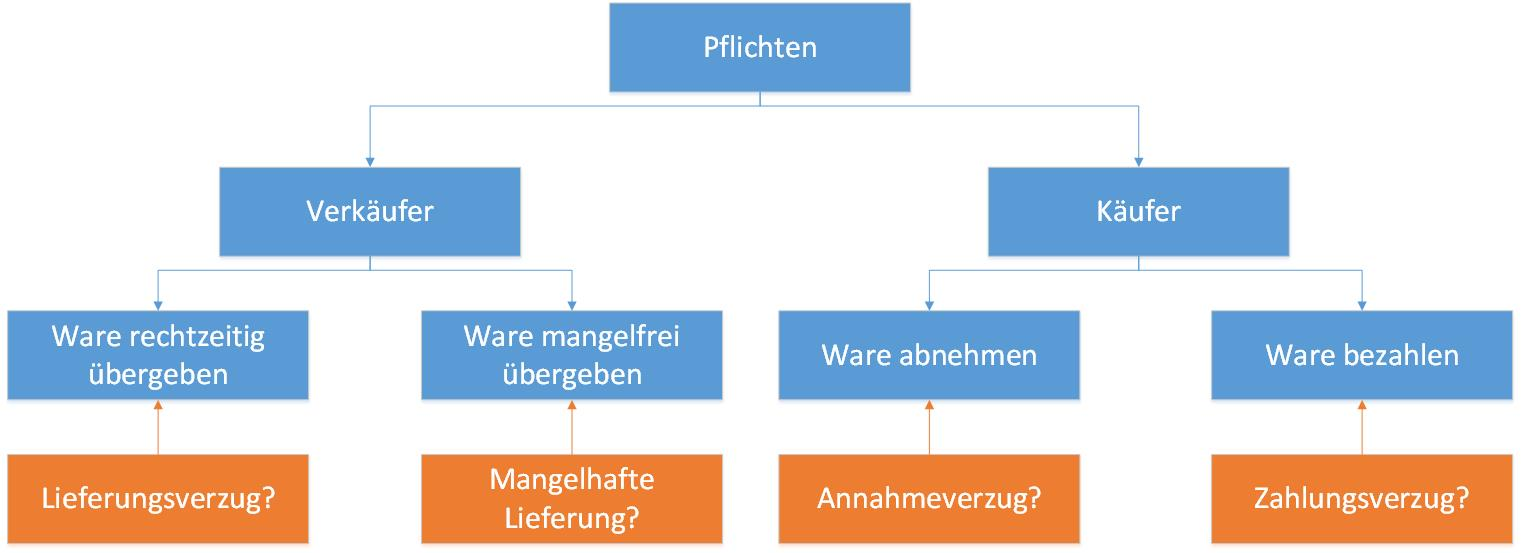
\includegraphics[scale=0.35]{pictures/lf01-pic/lf01-pflichten-kaufvertrag.jpg}

%%%Anfang: Beschaffungsprozess > Mangelhafte Lieferung
\subsubsection{Mangelhafte Lieferung}
Der Verkäufer verpflichtet sich mit dem Kaufvertrag, die Ware im vereinbarten Zustand zu liefern (§§434 ff. BGB: Der Verkäufer ist verpflichtet, die verkaufte Sache frei von Sach- und Rechtsmängeln zum Zeitpunkt des Gefahrenübergangs zu liefern [Gewährleistungspflicht].)

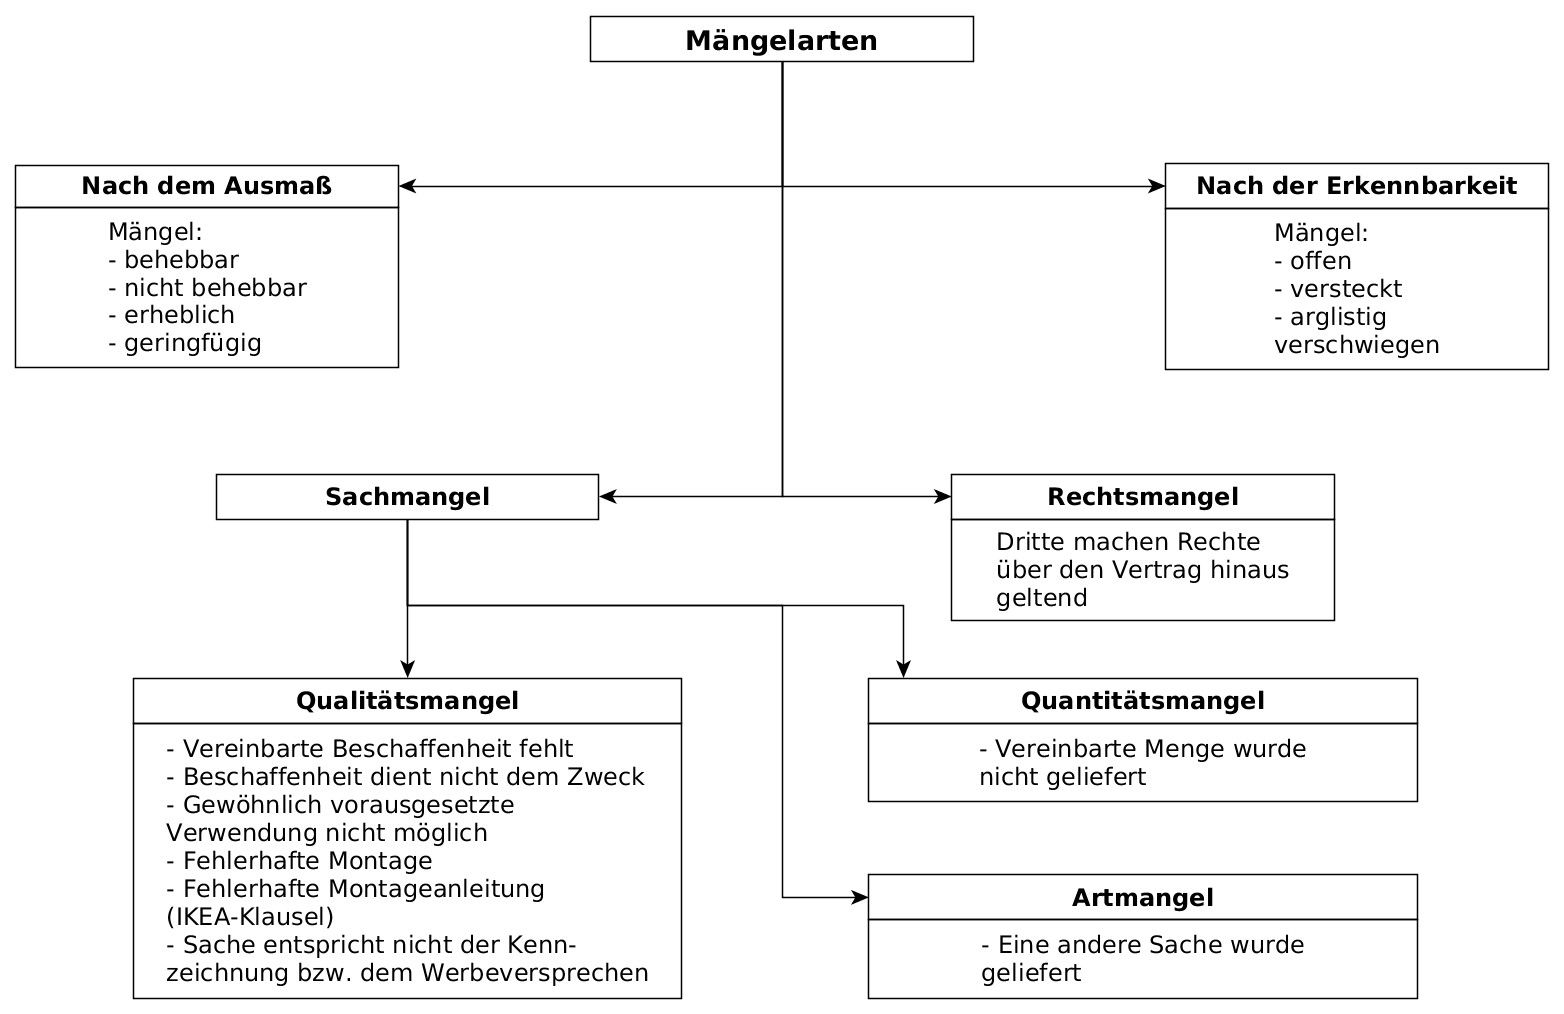
\includegraphics[scale=0.26]{pictures/lf01-pic/lf01-maengelarten.png}

%%%Anfang: Beschaffungsprozess > Mangelhafte Lieferung > Schuldfrage
\paragraph{Schuldfrage bei mangelhafter Ware (schlechter Leistung)}
	
\subparagraph{Hersteller} Der Hersteller hat die Verantwortung, wenn das Produkt nachweislich schon vor der Übergabe an den Lieferer mangelhaft war (versteckter Mangel). Der Lieferer kann gewährte Rechte (Zurücknahme, Minderung des Kaufpreises) gegen seinen Vorlieferer oder den Hersteller ohne Fristsetzung geltend machen. Zusätzlich kann ein angemessener Ersatz der Aufwendungen verlangt werden.

\subparagraph{Lieferer} Der Lieferer hat die Verantwortung zu tragen, wenn die Ware trotz eines offensichtlichen Mangels nicht beim Vorlieferanten gerügt wurde oder wenn der Mangel beim Lieferer entstanden ist. Ist dies der Fall, so muss der Lieferer für Mängel einstehen. Bei einem Verwendungskauf geht gemäß §447 BGB die Gefahr (das Transportrisiko) in dem Moment auf den Käufer über, in dem die mangelfreie Ware ordnungsgemäß verpackt und adressiert an den Frachtführer oder eine mit der Zusendung beauftragte Person übergibt.

\subparagraph{Frachtführer} Der Frachtführer muss die Verantwortung tragen, wenn sich der Schaden auf dem Transport ergab. Der Frachtführer muss für den Schaden haften, der Transportschaden muss jedoch nachgewiesen und dokumentiert werden.

\subparagraph{Kunde} Der Kunde muss die Verantwortung tragen, wenn er den Schaden nachweislich selbst herbeigeführt hat, den Schaden bei Vertragsabschluss kannte oder seine Rügepflichten nicht beachtet hat. Bei einem zweiseitigen Handelskauf hat der Kunde den Schaden selber zu tragen, außer der Verkäufer hat den Mangel arglistig verschwiegen oder eine Garantie für die Sache übernommen. Bei einem Verbrauchsgüterkauf findet in den ersten sechs Monaten nach dem Kauf eine Beweisumkehr statt. In dieser Zeit muss der Lieferer nachweisen, dass er mängelfrei geliefert hat.
	
%%%Anfang: Beschaffungsprozess > Mangelhafte Lieferung > Pflichten
\paragraph{Untersuchungs- und Rügepflicht des Käufers}

\subparagraph{Zweiseitiger Handelskauf} Bei einem zweiseitigen Handelskauf hat der Käufer die Ware sofort zu untersuchen und einen Mangel unverzüglich Anzuzeigen. Bei einer großen Warenmenge genügt auch die Überprüfung einer angemessenen Stichprobe. Wird nicht unverzüglich ein Mangel angezeigt, so gilt die Ware als genehmigt. Liegt ein versteckter Mangel vor, so muss der Käufer diesen unverzüglich nach der Entdeckung anzeigen.

\subparagraph{Einseitiger Handelskauf (Verbrauchsgüterkauf)} Der Verbraucher muss die Ware nicht unverzüglich untersuchen. Innerhalb von sechs Monaten hat der Verkäufer eine mangelfreie Lieferung nachzuweisen. Normaler Verschleiß und unsachgemäße Benutzung gehen auch in dieser Zeit zu Lasten des Verkäufers.Innerhalb von zwei Jahren kann der Verbraucher die gesetzlichen Gewährleistungsrechte in Anspruch nehmen, muss nach sechs Monaten aber nachweisen, dass der Mangel nicht durch normalen Gebrauch oder unsachgemäße Nutzung zustande gekommen ist. Die Gewährleistung kann bei gebrauchten Waren vom Verkäufer auf ein Jahr verkürzt werden.
	
%%%Anfang: Beschaffungsprozess > Mangelhafte Lieferung > Risiko
\paragraph{Gefahrenübergang/Transportrisiko}

\subparagraph{Versendungskauf} Beim Zweiseitigen Handelskauf und dem Privatverkauf ist der Erfüllungsort der Sitz des Verkäufers. Die Gefahr geht mit der Übergabe an den Frachtführer an den Kunden über. Der Kunde kann daher Anweisungen über die Art der Versendung erteilen. Diese Regelung besteht nicht, wenn der Verkäufer die Ware selbst zum Kunden transportiert (dann muss der Verkäufer bis zur Übergabe die Gefahr tragen). Der Kunde kann dem Frachtführer gegenüber Schadensersatz geltend machen.

\subparagraph{Verbrauchsgüterkauf} Beim einseitigen Handelskauf findet der Gefahrenübergang mit der Übergabe an den Käufer statt. Der Käufer trägt das Risiko des Transportes und kann daher die Verpackung und die Art der Beförderung wählen.

%%% Anfang: Beschaffungsprozess > Mangelhafte Lieferung > Rechte
\paragraph{Rechte des Käufers bei Mängeln}

\subparagraph{Nacherfüllung} Der Käufer kann zwischen der Beseitigung des Mangels (Nachbesserung) und der Lieferung einer mangelfreien Sache (Neulieferung) wählen. Die Transport-, Wege-, Arbeits- und Materialkosten hat dabei der Verkäufer zu tragen. Würde die geforderte Nacherfüllungsregelung für den Verkäufer unverhältnismäßig hohe Kosten verursachen, so kann er die geforderte Regelung verweigern. Der Kunde kann dann aber auf die andere Regelung Nacherfüllungsregelung bestehen.
	
\subparagraph{Rücktritt vom Kaufvertrag} Bestehen Sach- oder Rechtsmängel und sind mindestens zwei Nachbesserungsversucher fehlgeschlagen oder wird die Nacherfüllung verweigert, so hat der Kunde das Recht zum Rücktritt vom Kaufvertrag. Bestehen allerdings nur geringfügige Mängel, so besteht dieses Recht nicht.

\subparagraph{Minderung des Kaufpreises} Nach Frisetzung und Ablauf dieser Frist kann der Kunde auf eine Minderung des Kaufpreises bestehen. Diese Recht steht im auch bei geringfügigen Mängeln zu.

\subparagraph{Schadensersatz} Nach erfolgtem Rücktritt vom Kaufvertrag kann bei einer objektiven Pflichtverletzung aus dem Kaufvertrag, einer vorsätzlichen oder fahrlässigen Handlung des Verkäufers oder einer verstrichenen Nacherfüllungsfrist Schadensersatz gefordert werden. Dabei können die Leistungen des Kunden im Vertrauen auf die Nutzung der Ware und der Verzugsschaden geltend gemacht werden.

\subparagraph{Montageanleitung} Ist die Montageanleitung nicht einfach, klar und richtig formuliert (IKEA-Klausel), kann von einem Mangel an der Ware ausgegangen werden. Wird der vereinbarte Zusammenbau bei der Anlieferung vom Monteur nicht ordnungsgemäß durchgeführt, so kann auch dies reklamiert werden.

\subparagraph{Fernabsatzrecht} Das Fernabsatzrecht beinhaltet Haustürgeschäfte und den Internethandel. Grundsätzlich besteht für diese Geschäfte ein zweiwöchiges Widerrufs- und Rückgaberecht ohne Begründung. Der Verkäufer trägt die Kosten der Rücksendung, wenn der Preis der Ware 40\euro übersteigt und noch keine Gegenleistung in Form der Kaufpreiszahlung geleistet wurde. Bei mangelhafter Belehrung kann sich das Widerrufsrecht auf bis zu sechs Monate verlängern. Die Anbieter müssen über die Ware und deren Lieferbedingungen ausführlich informiert werden. Werden Waren ohne Bestellung geliefert, so brauchen diese nicht aufbewahrt oder zurückgeschickt werden. 
		
%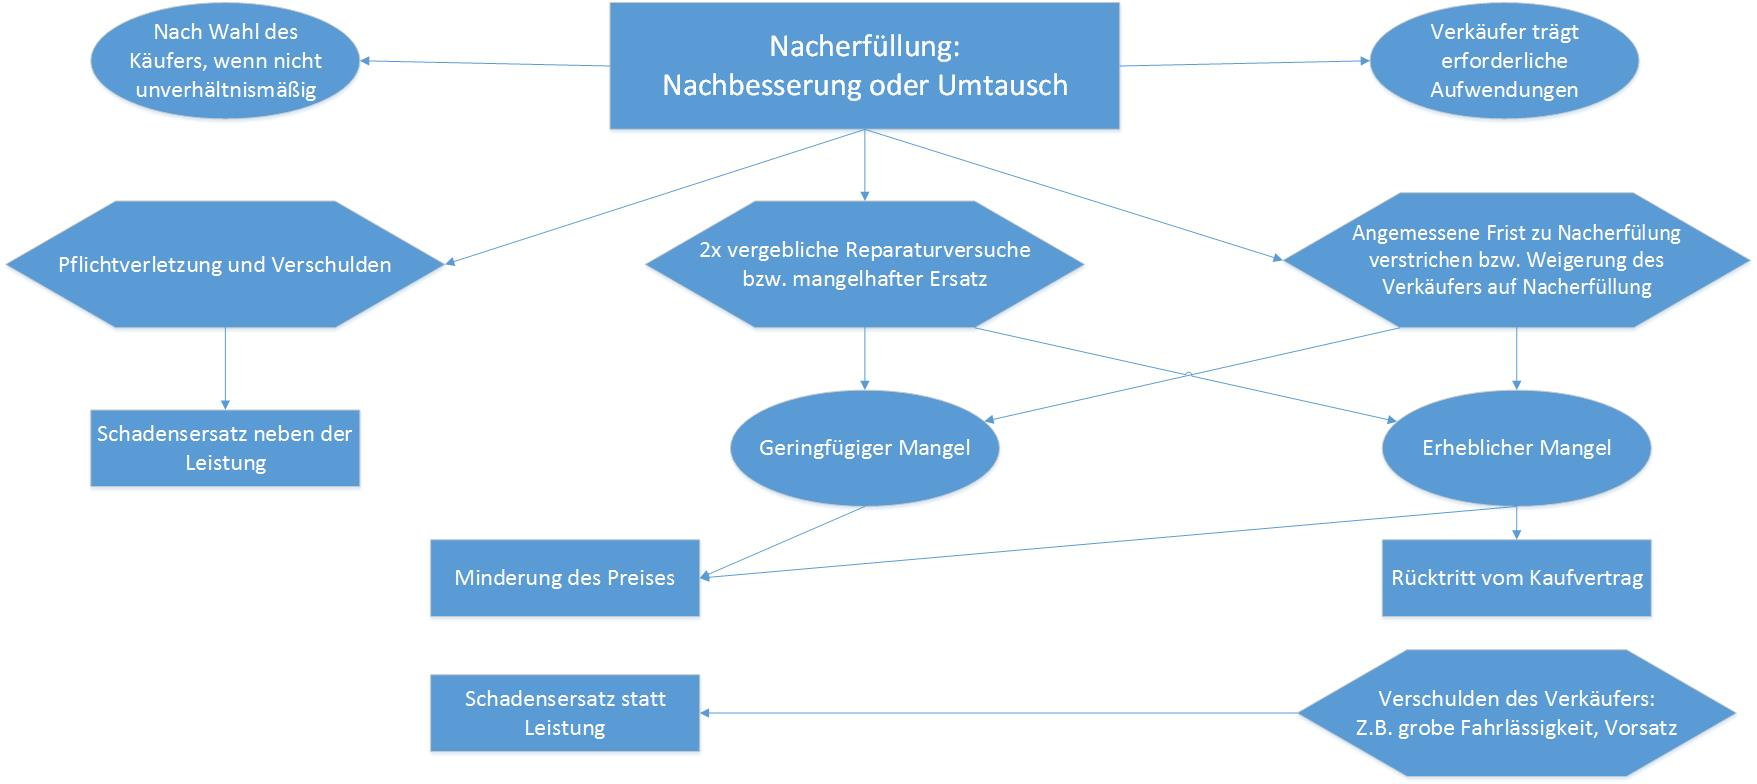
\includegraphics[scale=0.3]{pictures/lf01-pic/lf01-rechte_mangelhafte-leistung.jpg}\\
		
%%% Anfang: Beschaffungsprozess > Annahmeverzug
\subsubsection{Annahmeverzug}

\paragraph{Begriff}~\\
Ein Annahmeverzug liegt vor, wenn der Käufer die ordnungsgemäß gelieferte Ware (zur rechten Zeit am rechten Ort, mängelfrei) nicht annimmt. Ist hierbei jedoch keine genaue Leistungs- oder Lieferzeit bestimmt, so kommt der Käufer bei einer kurzzeitigen Abwesenheit nicht in Verzug. Der Leistungstermin muss vom Lieferanten eine angemessene Zeit vorher angekündigt werden.

\paragraph{Rechte des Verkäufers (Schuldners)}~\\
Der Verkäufer hat das Recht auf die Erfüllung des Vertrags. Daher kann er auf die Abnahme der Ware klagen. Die Ware kann er auf Kosten des Käufers hinterlegen (Dies betrifft unter Kaufleuten alle Gegenstände, beim Privatkauf nur Wertgegenstände). Weiterhin hat der Verkäufer das Recht auf einen Selbsthilfeverkauf durch öffentliche Versteigerung. Soweit es zeitlich möglich ist, muss diese dem Käufer jedoch vorab angedroht werden und er muss über den Termin und den Ort der Versteigerung unverzüglich informiert werden. Die Mehrkosten, die dem Verkäufer durch die Maßnahmen entstehen, kann er sich vom Käufer erstatten lassen. Nach einer Fristsetzung besteht zusätzlich die Möglichkeit eines Rücktritts vom Kaufvertrag.

\paragraph{Haftung für Waren nach dem Annahmeverzug}~\\
Der Verkäufer hat während des Annahmeverzugs des Käufers nur Vorsatz und grobe Fahrlässigkeit zu vertreten. Mit dem Annahmeverzug geht die Gefahr auch für Schäden durch Zufall auf den Käufer über.
	
%%% Anfang: Beschaffungsprozess > Lieferverzug
\subsubsection{Lieferverzug}

\paragraph{Voraussetzungen für Lieferverzug (nicht rechtzeitige Lieferung)}~\\
Ein Lieferverzug tritt ein, wenn die Frist des Liefertermins überschritten wird und eine Mahnung mit angemessener Nachfrist erfolglos geblieben ist. Zusätzlich muss der Lieferer den Verzug verschuldet haben. Dabei hat er auch das Verschulden seiner Erfüllungsgehilfen zu vertreten. Ein Lieferverzug tritt auch ohne Mahnung auf, wenn der Liefertermin kalendermäßig bestimmbar ist, die Lieferer die Leistung verweigert oder aus besonderen Gründen im beiderseitigen Interesse der sofortige Verzug gerechtfertigt ist.

\paragraph{Schadensersatz}~\\
Nachdem eine angemessene Nachfrist abgelaufen ist und eine erhebliche Pflichtverletzung des Verkäufers vorliegt, hat der Käufer das Recht auf Schadensersatz. Bei verzögerter Leistung muss der Verkäufer die zusätzlichen Aufwendungen ersetzten. Wenn auch eine Nachfrist keinen Erfolg bringt kann der Käufer Schadensersatz statt der Leistung fordern. Wird vom Verkäufer nur eine Teilleistung erbracht, so kann der Käufer nur Schadensersatz statt der ganzen Leistung verlangen, wenn er an der Teilleistung kein Interesse hat. Bereits geleistete Teilleistungen können dann vom Verkäufer zurückverlangt werden.

\paragraph{Konventionalstrafe}~\\
Käufer und Verkäufer können im Kaufvertrag eine Vertragsstrafe vereinbaren. Damit ersparen sich die Vertragspartner den Aufwand, einen eventuellen Schaden zu berechnen und haben vorab Klarheit über die Folgen im Falle des Verzugs. Konventionalstrafen werden häufig in Projektarbeiten verwendet.

\paragraph{sonstige Rechtsbestimmungen}~\\
Wird im Kaufvertrag kein Liefertermin genannt, so kann der Verkäufer sofort liefern und der Käufe die Lieferung sofort verlangen. Wenn offensichtlich ist, dass die Voraussetzungen für den Rücktritt vom Kaufvertrag eintreten werden, kann der Käufer bereits vor Eintritt der Fälligkeit zurücktreten. Vom ganzen Vertrag kann der Käufer jedoch nur zurücktreten, wenn er an der Teilleistung kein Interesse hat. Ist der Käufer weit überwiegend für den Verzug verantwortlich, so kann er nicht vom Vertrag zurücktreten.
	
%%% Anfang: Beschaffungsprozess > Zahlungsverzug
\subsubsection{Zahlungsverzug}

\paragraph{Voraussetzungen}~\\
Ein Zahlungsverzug tritt bei einer Fristüberschreitung des Zahlungstermins an. Ein Verzug entsteht ohne Mahnung, wenn der Termin kalendermäßig bestimmbar ist oder die Zahlung vom Käufer verweigert wird. Wenn nicht innerhalb von 30 Tagen nach Fälligkeit und Zugang der Rechnung gezahlt wird, tritt automatischer Zahlungsverzug ein. Ist dieser Zeitpunkt nicht feststellbar, so gilt Verzug spätestens nach Fälligkeit und Empfang der Gegenleistung. Ist der Zahlungstermin nicht kalendermäßig bestimmbar, so tritt Verzug ein, wenn gemahnt wurde. Verbraucher müssen auf die 30-Tage-Frist besonders hingewiesen werden. Der Käufer kommt nur in Verzug, wenn er das Unterbleiben der Leistung zu verschulden hat.
	
\paragraph{Rechte des Lieferers}~\\
Der Verkäufer kann ohne neue Fristsetzung auf eine nachträgliche Erfüllung des Kaufvertrags sowie auf Schadensersatz wegen Pflichtverletzung bestehen. Mit einer neuen Fristsetzung kann der Verkäufer vom Vertrag zurücktreten (der Käufer muss die Leistung zurückgeben) sowie Schadensersatz statt Zahlung fordern.
	
\paragraph{Verzugszinsen} ~\\
Der Verzugszinssatz beträgt für das Jahr fünf Prozentpunkte über dem Basiszinssatz. Ist in dem Rechtsgeschäft kein Verbraucher involviert, beträgt der Verzugszinssatz acht Prozentpunkte über dem Basiszinssatz. Der aktuelle Basiszinssatz liegt bei -0,83\%. Bei der Berechnung der Tage wird nach der {\it Eurozinsmethode} vorgegangen. Danach wird jeder Monat kalendergenau und jedes Jahr mit 360 Zinstagen berechnet.

%%% Ende: Beschaffungsprozess
%%%%%%%%%%%%%%%%%%%%%%%%%%%%%%%%%%%%%%%%%%%%%%%%%%%%%%%%%%%%%%%%%%%%%%%%%%%%%%%%